\chapter{Marco Teórico}
\section{Vientos Estelares}
\section{Choques}
\section{Frentes de Ionización}
Un frente de ionización es la interfaz entre un medio gaseoso neutro y uno
ionizado. Ocurren cerca de fuentes de rediación ionizante, tales como
estrellas masivas, tipo B temprana o tipo O. el frente de ionización puede
tratarse como una discontinuidad en el medio gaseoso.

\section{Regiones HII \citep{Stahler:2004}}
\label{sec:HII}
\newcommand\Nio{\ensuremath{\mathcal{N}}}
%\newcommand\N{\ensuremath{\mathcal{N}}}

Consideremos el caso en que se forma una estrella masiva dentro de una nube molecular, que por simplicidad está compuesta exclusivamente de hidrógeno molecular $H_2$. La estrella masiva emite fotones ultravioleta que tienen la energía suficiente para disociar el $H_2$  como para ionizar el hidrógeno atómico resultante. Luego el plasma ionizado se recombina para volver a ser $HI$ emitiendo líneas espectrales de diversas energías, siendo la más energética la línea de $\mathrm{Ly~}\alpha$. Como al realizar una ionización se pierde un fotón ionizante y el flujo de radiación proveniente de la estrella es finito, entonces la estrella solo puede ionizar la región de la nube más próxima a ésta. Si suponemos que la nube tiene densidad uniforme, entonces esta región tendrá forma esférica, conocida como \textit{esfera de Strömgren}.

\subsection{Esfera de Strömgren}

El plasma ionizado dentro de la Esfera de Strömgren se encuentra en balance de ionización, esto es, que la tasas de ionización y la de recombinación son iguales. La tasa de ionizaciones es igual a la cantidad de fotones ionizantes que emite la estrella central por segundo. Esto es, los fotones que poseen una energía mayor al límite de Lymann, que corresponde a  $E = 13.6\mathrm{~eV}$, o bien $\lambda = 912\mathrm{~\AA}$. En la tabla \ref{tab:ionizing-radiation} se muestra la tasa de fotones ionizantes $\Nio_*$ para estrellas masivas de tipo espectral O y B temprano.

\begin{table}
  \begin{tabular}{cccc} \hline 
    Tipo & Masa & $\log \Nio_*$ & \log \Nio_{FUV} \\
    Espectral & $(M_\odot)$ & $(s^{-1})$ & $(s^{-1})$  \\
    \hline
    O4 & 70 & 49.9 & 49.5 \\
    O5 & 60 & 49.4 & 49.2 \\
    O6 & 40 & 48.8 & 48.8 \\
    O7 & 30 & 48.5 & 48.6 \\
    O8 & 23 & 48.2 & 48.4 \\
    O9 & 20 & 47.8 & 48.2 \\
    B0 & 18 & 47.1 & 48.1 \\
    B1 & 13 & 45.4 & 47.5 \\
    B2 & 10 & 44.8 & 47.1 \\
    \hline
  \end{tabular}
  \caption{Tasa de fotones ionizantes para estrellas masivas \citep{Stahler:2004}}
  \label{tab:ionizing-radiation}
\end{table}

Por otro lado, la tasa volumétrica de recombinaciones se escribe como:

\begin{align}
  \ensuremath{\mathcal{R}} = n_e n_p \alpha_{rec}(T) = n^2_e \alpha_{rec}(T)
\end{align}

Donde $\alpha_{rec}$ es el \texit{coeficiente de recombinación}, y es una función solo de la temperatura. La última iguladad se obtiene asumiendo neutralidad de la carga.

La tasa total de recombinaciones se obtiene integrando $\ensuremath{\mathcal{R}}$ en el volumen de la región $HII$, asumiendo que tanto la densidad de electrones como la tempertaura son constantes espacialmente. De esta manera la condición de balance de ionización queda como sigue:

\begin{align}
  \Nio_* = \frac{4\pi}{3} n^2_e \alpha'_{rec}(T)R^3_s 
\end{align}

Donde $R_s$ es el \textit{radio de Strömgren}. Es importante notar que el coeficiente de recombinación primado es diferente del coeficiente no primado: el coeficiente de recombinación primado no toma en cuenta las recombinaciones al nivel $n = 1$ debido a que estas recombinaciones producen fotones de $E = 13.6\mathrm{~eV}$ que son capaces de ionizar el hidrógeno neutro.

Como la densidad de la nube original no cambia apreciablemente cuando el gas es ionizado debido a que el tiempo en que esto pasa es muy corto (como mostraremos en la siguiente sección), entonces $n_e = n^0_H$, donde $n^0_H$ es la densidad de $HI$ en la región contigua a la nube, y a su vez $n^0_H = n_{H_2}$, donde $n_{H_2}$ es la densidad de gas molecular. Con esto podemos calcular el radio de Strömgren como sigue:

\begin{align}
  R_s = \left[\frac{3\Nio_*}{4\pi\alpha'_{rec}(n^0_H)^2}\right]^{1/3} = 0.4\mathrm{~pc}\left(\frac{\Nio_*}{10^{49}\mathrm{~s^{-1}}}\right)^{1/3}\left(n_{H_2}\right)^{-2/3}
\end{align}

En la expresión numérica, se adopta un valor de $\Nio_*$ de $10^{49}\mathrm{s^{-1}}$, una temperatura de $10^4\mathrm{~K}$ que es la temperatura característica de una región $HII$ y con la que el coeficiente de recombinación $\alpha'_{rec}$ adopta un valor de $2.6\times 10^{-13}\mathrm{~cm^3~s^{-1}}$.

Dentro de la región $HII$, la probabilidad por unidad de tiempo de ionizar un átomo de hidrógeno dado es mucho mayor a la probabilidad de una recombinación, por lo que el gas está casi completamente ionizado. Sin embargo, en los bordes de la región $HII$, la densidad de gas neutro aumenta debido a que en dicha región el flujo de fotones ionizantes ha sido atenuado por todo el gas ionizado más próximo a la estrella. La transición de gas ionizado a gas neutro tiene un grosor $\Delta r$ que corresponde al camino libre medio del gas neutro. Esto es:

\begin{align}
\Delta R = \frac{1}{\sigma_{\nu_1}n^0_H}  
\end{align}

Donde $\sigma_{\nu_1}$ es la sección recta de un átomo de hidrógeno en el estado base, evaluada en la longitud de onda del límite de Lymann. Utilizando $\sigma_{\nu_1} = 6.8\times 10^{-18}\mathrm{~cm^2}$ y $n^0_H = 2\times 10^{3}\mathrm{~cm^{-3}}$ obtenemos que $\Delta r = 7.4\times 10^{13}\mathrm{~cm} \sim 5\times 10^{-5}~R_s$, lo que muestra que las regiones $HII$ tienden a tener bordes bien delimitados.

\subsection{Primera y Segunda expansión}

Las esferas de Strömgren no son objetos estáticos, sino que se expanden con el tiempo. Este proceso ocurre en dos etapas: en la primera inicialmente no existe ninguna región $HII$ pero que la radiación ultravioleta de la estrella hace que se expanda rápidamente al disociar e ionizar el gas a su alrededor hasta alcanzar el radio de Strömgren. En la segunda expansión la diferencia de presiones entre el gas ionizado de la región $HII$, mucho mayor que la del gas neutro que lo rodea, provoca otra expansión más lenta que la primera hasta que haya equilibrio de presión. A continuación explicaremos el proceso más a detalle:

Sea $F_*(t)$ el flujo de radiación ionizante que alcanza un radio $R$ al tiempo $t$. Al transcurrir un tiempo $dt$, el frente de ionización avanza una distancia $dR$ y llega a $n^0_{H_2}$ moléculas de hidrógeno por unidad de área. Se necesitan 3 fotones para ionizar completamente la molécula: uno para disociarla, con energía $E\geq 14.7\mathrm{~eV}$ y otros dos para ionizar cada uno de los átomos resultantes, con $E\geq13.6\mathrm{~eV}$. El número de fotones ionizantes atravezando el frente de ionización por unidad de área es $F_*~dt$. Entonces, como se producen dos ionizaciones por cada tres fotones (Figura \ref{fig:ionization}), tenemos que:

\begin{align}
  \frac{F_* dt}{2 n_{H_2} dR} &= \frac{3}{2} \\
  \implies \frac{dR}{dt} &= \frac{F_*}{3n_{H_2}} = \frac{2 F_*}{3 n^0_H}
\end{align}

\begin{figure}
  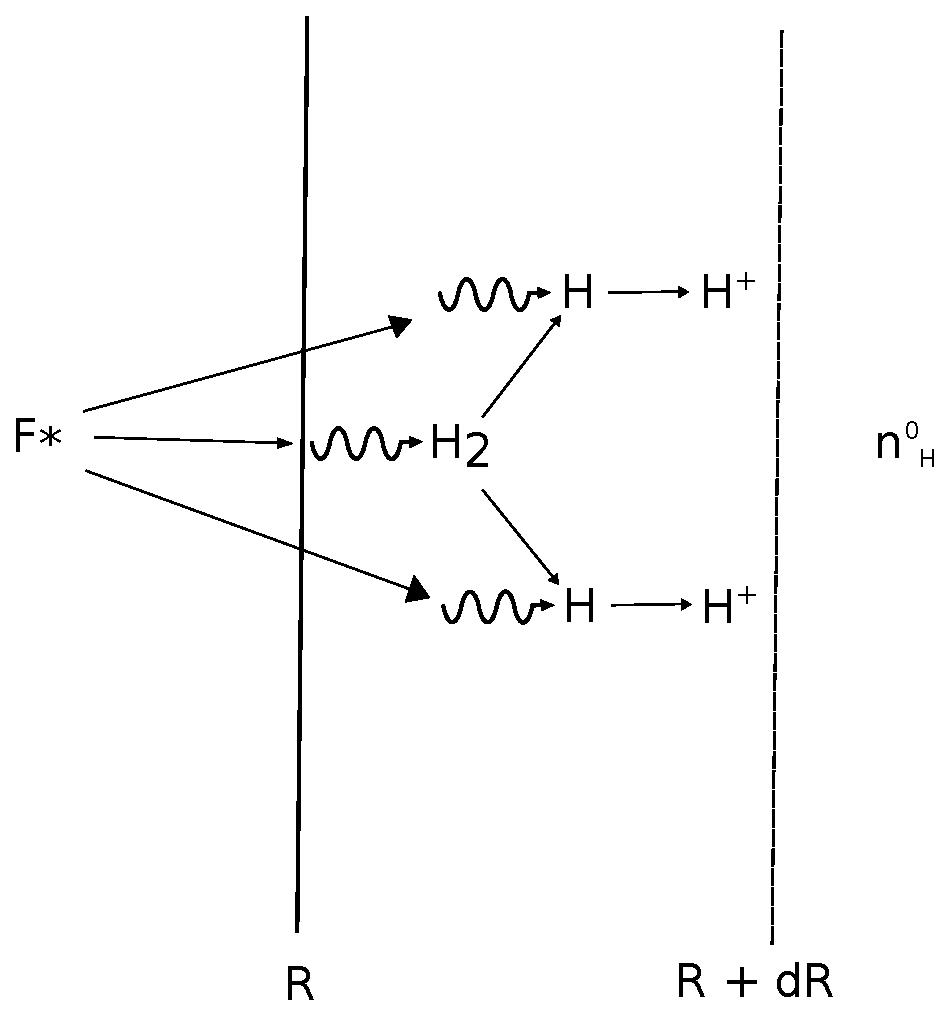
\includegraphics[width=0.6\linewidth]{./Figures/ionization}
  \caption{Representación de la primera expansión del frente de ionización de una región $HII$ con densidad numérica del hidrógeno $n^0_H$. De cada tres fotones ionizantes que cruzan el frente en R, uno disocia una molécula de hidrógeno y los otros dos ionizan los átomos resultantes \citep{Stahler:2004}}
  \label{fig:ionization}
\end{figure}


Estamos asumiendo que el flujo tanto de fotones con energías de $E\geq 14.7\mathrm{~eV}$ y $E\geq 13.6\mathrm{~eV}$ es prácticamente el mismo.

Ahora consideremos las recombinaciones: el número total de recombinaciones que llevan a niveles tales que $n \geq 2$ dentro de una esfera de radio $R$ es $\frac{4\pi}{3}\left(n^0_H\right)^2\alpha'_{rec}R^3$. Si el balance de ionización aun se mantiene, entonces el número de ionizaciones por unidad de tiempo es igual a la tasa de recombinaciones más los fotones que logran atravesar el frente de ionización por unidad de tiempo que es $4\pi R^2 F_*$. Entonces:

\begin{align}
  \Nio_* = 4\pi R^2 F_* + \frac{4\pi}{3}\left(n^0_H\right)^2\alpha'_{rec}R^3
\end{align}

Resolvemos para $F_*$ y encontramos que:

\begin{align}
  F_* &= \frac{\Nio_*}{4\pi R^2} - \frac{\left(n^0_H\right)^2\alpha'_{rec} R}{3} \\
  \implies \frac{dR}{dt} &= \frac{\Nio_*}{6\pi n^0_H R^2} - \frac{2n^0_H \alpha'_{rec} R}{9} \label{eq:1-expansion-eq} 
\end{align}

Definimos los siguientes parámetros adimensionales $\lambda \equiv R/R_s$ y $\tau \equiv t/t_{rec}$, donde $t_{rec} = \frac{1}{n^0_H \alpha'_{rec}}$ es el tiempo medio de recombinación del hidrógeno, que es del órden de $60\mathrm{~yr}$ con los valores de $n^0_H$ y $\alpha'_{rec}$ utilizados en esta sección. Y con esto la ecuación (\ref{eq:1-expansion-eq}) se escribe como sigue:

\begin{align}
  \frac{d\lambda}{d\tau} = \frac{2}{9}\left(\lambda^{-2} - \lambda\right) \label{eq:d-lambda-tau}
\end{align}

Resolvemos por el método de separación de variables y aplicamos la condición inicial $\lambda(0) = 0$ y obtenemos lo siguiente:

\begin{align}
  \lambda(\tau) = \left[1 - \exp\left(-\frac{2}{3}\tau\right)\right]^{1/3} \label{eq:lambda-tau}
\end{align}

De la ecuación (\ref{eq:lambda-tau}) vemos que cuando han pasado una y media veces del tiempo de recombinación,  la región $HII$ se ha expandido alrededor del $86\mathrm{\%}$ del radio de Strömgren, y aunque la expansión se va descelerando constantemente, ya es de una extensión considerable.

La velocidad del sonido en el gas ionizado con temperatura de $\sim 10^4\mathrm{K}$ es de $a_{II}\sim 10\mathrm{km~s^{-1}}$, si comparamos esta velocidad con la media de la velocidad del frente de ionización, por ejemplo, en el intervalo $0< \tau < \frac{3}{2}$, en el que ya comprobamos que el frente de ionización casi alcanza el radio de Strömgren, encontramos lo siguiente:

\begin{align}
  \bar{v}_{IF} = \frac{R_s}{t_{rec}}\frac{1}{\frac{3}{2}- 0}\int^{\frac{3}{2}}_0 \frac{d\lambda}{d\tau}~d\tau = \frac{2R_s}{3t_{rec}}\lambda\left(3/2\right)
\end{align}

Con los valores típicos adoptados en esta sección obtenemos que:

\begin{align}
  \bar{v}_{IF}\simeq 135\mathrm{~km~s^{-1}}\left(\frac{\Nio_*}{10^{49}\mathrm{~s^{-1}}}\right)^{1/3}\left(n_{H_2}\right)^{-2/3}
\end{align}
Dado que la velocidad media del IF es mucho mayor que la del sonido del gas ionizado, entonces es razonable asumir que la densidad del gas ionizado es igual a la del gas neutro dado que la densidad del gas no tiene tiempo de reajustarse después de ser ionizado. Sin embargo, la presión sí se vuelve mucho mayor en el gas ionizado que en el gas neutro, y este gas empieza a generar una segunda expansión más lenta que la primera, que provoca que la densidad del gas ionizado disminuya, hasta que llega a un equilibrio de presión con el gas neutro circundante.
\subsection{Flujos de Champaña}
\subsection{Características de la emisión}
% Las regiones HII se forman cuando una estrella masiva, de tipo espectral O ó B temprana, ioniza el gas que se encuentra a su alrededor. El gas ionizado se encuentra en equilibrio térmico, a una temperatura del orden de $10^4~\mathrm{K}$. El principal proceso de calentamiento es la radiación de la estrella central, mientras que el enfriamiento se da principalmente por la recombinación de líneas prohibidas y por emisión libre-libre.

\section{Modelo Genérico de los Choques de Proa}
\label{sec:Modelo-generico}
Para este trabajo consideramos en general dos modelos de
interacción  de vientos:
\begin{itemize}
\item Una fuente localizada en el origen que emite un viento esférico
  que puede ser isotrópico o anisotrópico (figura
  \ref{fig:isotropic-aniso}) no acelerado que interactúa con el viento
  esférico isotrópico de otra fuente que se encuentra a una distancia
  $D$ de la primera(figura \ref{fig:crw-esquema})
\item Una fuente localizada en el origen que emite un viento esférico
  isotrópico no acelerado que interactúa con un viento plano paralelo
  no acelerado y densidad constante (figura )
\end{itemize}
El sitema en su conjunto tiene simetría cilíndrica.
\begin{figure}
  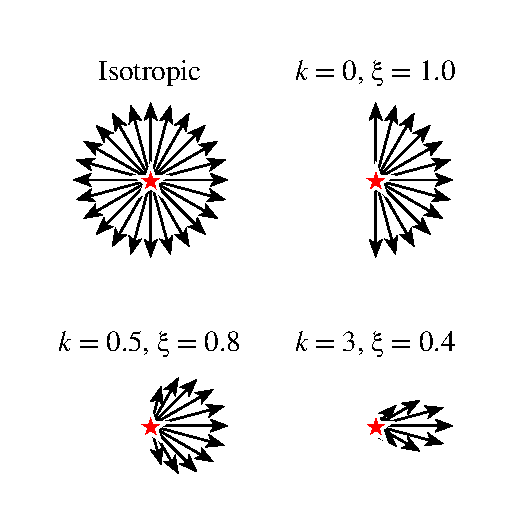
\includegraphics[width=0.5\linewidth]{./Figures/anisotropic-arrows}
  \caption{Representación esquemática de vientos con diferentes
    anisotropías:
    Arriba izquierda: Viento isotrópico esférico. Arriba derecha: viento
    isotrópico hemisférico. Abajo: Vientos anisotrópicos donde el
    parámetro $k$ indica el grado de anisotropía (ver capítulo \ref{chap:hipersonica})}
    \label{fig:isotropic-aniso}
\end{figure}
\begin{figure}
  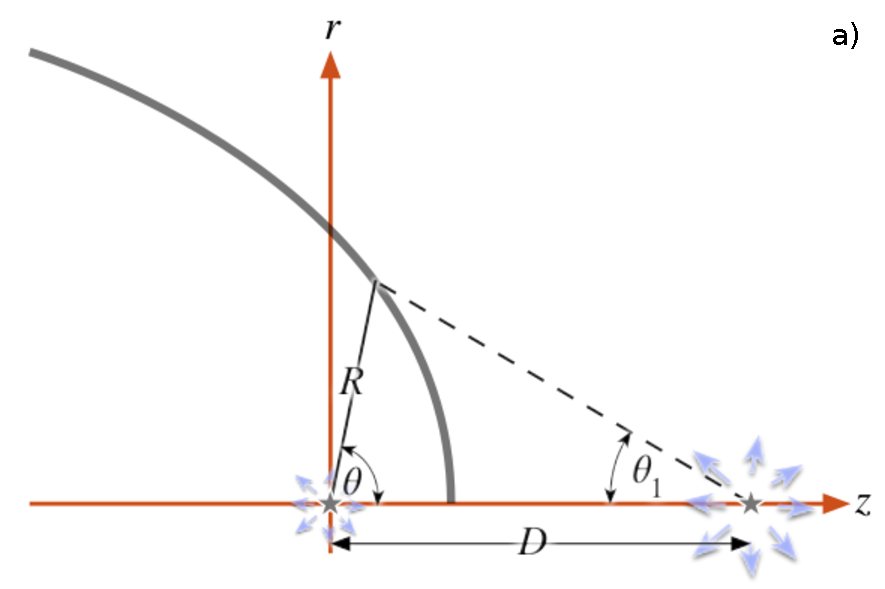
\includegraphics[width=0.5\linewidth]{./Figures/bowshock-crw-variables}
  \caption{Representación esquemática del problema de interacción de dos vientos:
    Dos fuentes separadas por una distancia $D$ emiten un viento radial que forma un
    choque de proa a una distancia $R$ del origen. El sistema tiene geometría cilíndrica
    siendo el eje $z$ el eje de simetría. La forma del choque depende únicamente del ángulo
    polar $\theta$, medido a partir del origen. Otro ángulo que es de utilidad es $\theta_1$,
    que corresponde al ángulo polar medido a partir de la posición de la otra fuente.}
    \label{fig:crw-esquema}
\end{figure}

\subsection{Planitud y ``Alatud''}
\label{sec:char-rad}
Las cantidades medibles que nos ayudan a caracterizar un choque de proa las
llamamos ``Radios característicos'' (ilustrados en la figura
\ref{fig:char-radii}):
\begin{itemize}
\item Radio del choque en la dirección del eje de simetría del sistema.
  Denotado como $R_0$
\item Radio en dirección perpendicular al eje de simetría del sistema.
  Denotado como $R_{90}$
\item Radio de curvatura en la ``nariz'' del choque de proa. Denotado
  como $R_c$. En el apéndice \ref{app:math-curvature-radius} se muestra
  el procedimiento para obtener este radio para una curva genérica continua
  y derivable.
\end{itemize}

\begin{figure}
  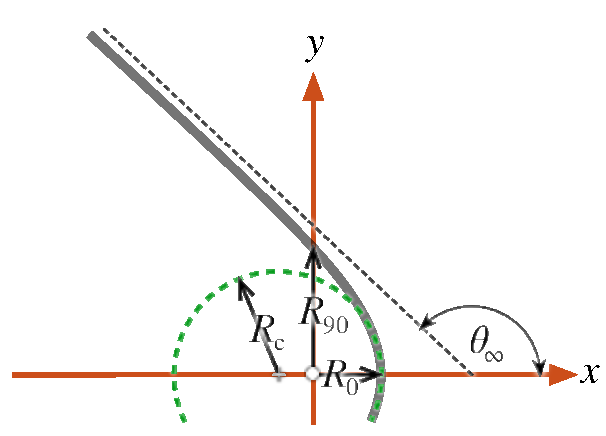
\includegraphics[width=0.5\linewidth]{./Figures/characteristic-radii}
  \caption{Representación esquemática de los radios característicos
    de un choque de proa}
  \label{fig:char-radii}
\end{figure}
Un último parámetro es el ángulo asintótico de apertura de las alas, denotado como $\theta_\infty$. Sin embargo, en la mayoría de los choques de proa es dificil de medirlo debido a que el ángulo polar $\theta$ tiende al valor asintótico muy lentamente y además la emisión de las alas es bastante débil. Por otro lado, los radios característicos $(R_0, R_c, R_{90})$ son medibles observacionalmente en la mayoría de los casos. A partir de éstos, podemos determinar dos parámetros adimensionales llamados ``planitud'' y ``alatud''. El primero de éstos es una medida de qué tan plano es el choque de proa en la nariz o ``apex'', y lo denotamos con la letra griega $\Pi$, mientras que el segundo es una medida de qué tanto se abren las alas del choque de proa, y lo denotamos con la letra griega $\Lambda$. Ambos parámetros se definen a continuación:

\begin{align}
  \Pi \equiv \frac{R_c}{R_0} \\
  \Lambda \equiv \frac{R_{90}}{R_0}
\end{align}

  
%Para este trabajo resulta útil hacer una noramlización de los radios
%característicos u otros radios, para que las mediciones que obtengamos
%sean adimensionales. De esta forma, podemos hacer la normalización con
%la distancia $D$, o bien con $R_0$, dependiendo de qué tipo de
%normalización resulte más conveniente. En el primer caso expresamos
%explícitamente el cociente (e.g $\frac{R_0}{D}$, $\frac{R_c}{D}$,
%$\frac{R_{90}}{D}$), y en el segundo caso añadiremos una tilde al
%radio en cuestión (e.g $\tilde{R}_c$, $\tilde{R}_{90}$). 

\section{Proyección en el Plano del Cielo}
\label{sec:projection}

Para un choque de proa que es la vez geométricamente delgado y
ópticamente delgado, únicamente se observa el borde de éste por
abrillantamiento al limbo, por lo tanto, su orientación respecto a
la línea de visión modifica su forma respecto a la forma real del
choque. Para ello, rotamos el sistema de referencia del choque de proa
en coordenadas cartesianas, denotado por $(x, y, z)$, por un ángulo
que llamamos \textit{inclinación}, denotado por $i$, en el plano $xz$,
de modo que la transformación entre el sistema de refencia del choque
y el sistema de referencia del plano del cielo, denotado por
$(x', y', z')$ queda como sigue:

\begin{align}
  \left(
  \begin{array}{c}
    x' \\ y' \\ z'
  \end{array}
  \right) &=
  \left(
  \begin{array}{c}
    x\cos i - z\sin i \\ y' \\ z\cos i + x\sin i
  \end{array}
  \right)
  \label{eq:rotation}
\end{align}

Por otro lado, la forma tridimensional del choque de proa viene dado por:

\begin{align}
  \left(
  \begin{array}{c}
    x \\ y \\ z
  \end{array}
  \right) &=
            R(\theta)\left(
            \begin{array}{c}
              \cos\theta \\
              \sin\theta\cos\phi \\
              \sin\theta\sin\phi
            \end{array}
            \right)
\end{align}
La relación entre ambos sistemas de referencia se ilustra en la figura
\ref{fig:reference}.

\begin{figure}
  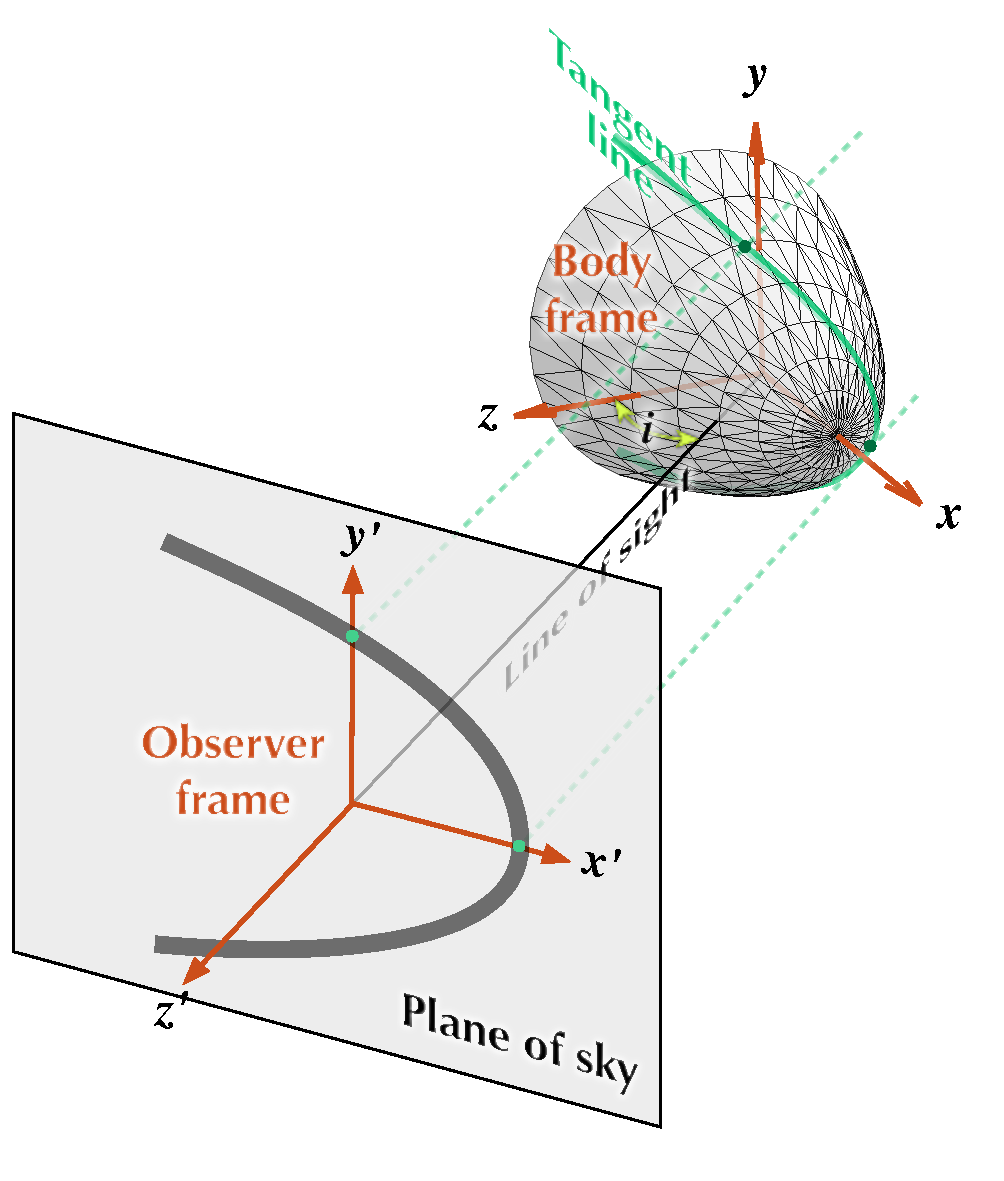
\includegraphics[width=0.5\linewidth]{./Figures/projection-pos}
  \label{fig:reference}
  \caption{Sistema de referencia del choque vs sistema de referencia del
    plano del cielo. Los ejes $x'$ y $y'$ se encuentran en el plano del
    cielo, mientras el eje $z'$ es paralelo a la línea de visión.
    Solo la regi\'on del choque cuya tangente sea paralela a la l\'inea
    de visión será visible por abrillantamiento al limbo.}
\end{figure}

\subsection{Vectores normal y tangente a la superficie}

Si definimos los vectores $\hat{n}$ y $\hat{t}$, como los vectores
normal y tangente a la superficie, respectivamente para $\phi$ constante.
En el caso $\phi = 0$ (figura \ref{fig:unit-vec}), ambos vectores se encuentran
en el plano $xy$ y es fácil mostrar que:

\begin{align}
  \hat{t}_0 =
  \left(
  \begin{array}{c}
    -\cos\alpha \\
    \sin\alpha \\
    0
  \end{array}
  \right)
  \quad \mathrm{y} \quad
  \hat{n}_0 =
  \left(
  \begin{array}{c}
    \sin\alpha \\
    \cos\alpha \\
    0
  \end{array}
  \right)
  \label{eq:unit-vec}
\end{align}

Donde:
\begin{align}
  \tan\alpha = -\frac{dy}{dx} = \frac{1+\omega\tan\theta}{\tan\theta-\omega}
\end{align}
y:
\begin{align}
  \omega(\theta) = -\frac{1}{R}\frac{dR}{d\theta} 
\end{align}

Para otros valores de $\phi$, basta con hacer una rotación de las ecuaciones
(\ref{eq:unit-vec}) alrededor del eje $x$. Para la conversión al sistema de
referencia del plano del cielo se utiliza la ecuación (\ref{eq:rotation}):

\begin{align}
\begin{split}
  \hat{n}' &= \frac{1}{\left(1 + \omega^2\right)^{1/2}} \\
           & \times \left(
             \begin{array}{c}
               (\cos\theta+\omega\sin\theta)\cos i-(\sin\theta-\omega\cos\theta)\sin i\sin\phi\\
               (\sin\theta-\omega\cos\theta)\cos\phi \\
               (\cos\theta+\omega\sin\theta)\sin i+(\sin\theta-\omega\cos\theta)\sin\phi\cos i
             \end{array}
                    \right) \\
\end{split}\\
\begin{split}
    \hat{t}' &= \frac{1}{\left(1 + \omega^2\right)^{1/2}} \\
           & \times \left(
             \begin{array}{c}
               -(\sin\theta-\omega\cos\theta)\cos i-(\cos\theta+\omega\sin\theta)\sin i\sin\phi\\
               (\cos\theta+\omega\sin\theta)\cos\phi \\
               -(\cos\theta+\omega\sin\theta)\sin i+(\sin\theta-\omega\cos\theta)\sin\phi\cos i
             \end{array}
             \right)
\end{split} 
\end{align}


\begin{figure}
  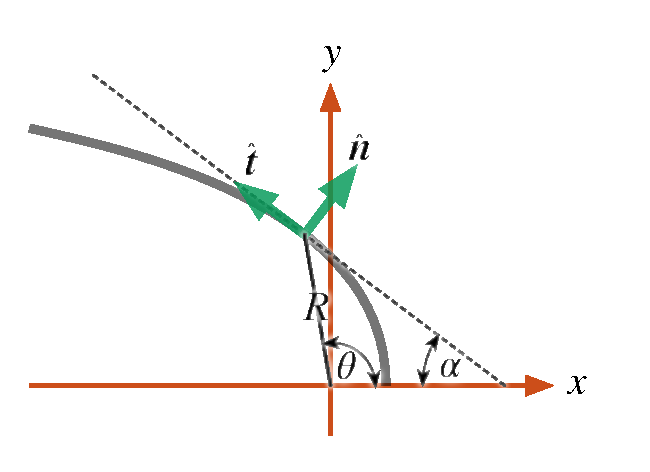
\includegraphics[width=0.6\linewidth]{./Figures/bowshock-unit-vectors}
  \caption{Vectores unitarios normal y tangente a la superficie $R(\theta)$
    en un plano de azimuth $\phi$ constante.}
    \label{fig:unit-vec}
\end{figure}


\subsection{Línea tangente}
\label{sec:tangent-line}
Debido a que el choque es ópticamente delgado y geométricamente
delgado, solo la región del choque cuya tangente sea paralela a la
línea de visión seré visible. Esto corresponde a una curva que
denominamos \textit{línea tangente}, que debe cumplir con la siguiente
condición:

\begin{align}
  \hat{n}'\boldsymbol{\cdot} \hat{z}' = 0
\end{align}

Denotamos como $\phi_T$ al ángulo azimutal que cumple la condición anterior
para una inclinación dada, en función del ángulo polar $\theta$:
\begin{align}
  \sin\phi_T = \tan i\tan\alpha = \tan i\frac{1+\omega\tan\theta}{\omega-\tan\theta}
  \label{eq:phi-tan}
\end{align}
De esta manera, la forma de la línea tangente del choque de proa, a la que llamamos
\textit{forma proyectada} viene dada por:

\begin{align}
  \left(
  \begin{array}{c}
    x'_T \\
    y'_T \\
    z'_T
  \end{array}
  \right) =
  R(\theta)\left(
  \begin{array}{c}
    \cos\theta\cos i - \sin\theta\sin\phi_t\sin i \\
    \sin\theta\left(1-\sin^2\phi_T\right)^{1/2} \\
    \cos\theta\sin i + \sin\theta\sin\phi_T\cos i
  \end{array}
  \right) \label{eq:proj-shape}
\end{align}
En el caso general, $z'_T$ no es una función lineal de $x'_T$ y $y'_T$, por lo que
la línea tangente no se encuentra en un plano.

La forma aparente $(x'_T, y'_T)$  de la línea tangente también puede escribirse
en coordenadas polares $(R', \theta')$, donde:
\begin{align}
  R'(\theta) = \left(x'^2_T + y'^2_T\right)^{1/2} & \mathrm{y} & \tan\theta' = \frac{y'_T}{x'_T}
  \label{eq:polar}
\end{align}
Es de notar a su vez que la ecuación (\ref{eq:phi-tan}) no tiene solución para valores
arbitrarios de $\theta$ y de la inclinación, puesto que se requiere que
$\left|\sin\phi_T\right| < 1$. Por tanto, la línea tangente solo existe para valores
de $\theta$ tales que $\theta < \theta_0$ donde $\theta_0$ es el valor de $\theta$ en
el eje de simetría de la línea tangente proyectada $(\theta'(\theta_0) = 0)$ y que se
obtiene de la siguiente ecuación implícita:
\begin{align}
  \tan\theta_0 = \frac{|\tan i| + \omega(\theta_0)}{1 - \omega(\theta_0)|\tan i|}
  \label{eq:th-0}
\end{align}
Esto implica que si el choque de proa es suficientemente ``abierto''
$(\alpha > \alpha_{min})$, entonces para inclinaciones tales que
$|i| > 90^\circ - \alpha_{min}$ no existirá la línea tangente para ningún valor de $\theta$,
es decir, el choque de proa se encontrará sufientemente ``de cara'' como para que ya no
parezca un choque de proa para el observador.

\subsection{Radios característicos en el plano del cielo}

En orden de comparar la forma $R(\theta)$ con observaciones, es útil definir los radios
característicos $R'_0$ y $R'_{90}$, donde $R'_0$ es el radio del eje de simetría aparente
y $R'_{90}$ es el radio aparente en la dirección perpendicular a $R'_0$. Es decir
$R'_0 = x'_T(y'_t=0)$ y $R'_{90} = y'_t(x'_t = 0)$. Utilizando las ecuaciones
(\ref{eq:phi-tan}) y (\ref{eq:proj-shape}) encontramos que:
\begin{align}
R'_0 = R(\theta_0)\cos(\theta_0 + i)
\label{eq:R0p}
\end{align}
Donde $\theta_0$ es la solución de la ecuación (\ref{eq:th-0}), y
\begin{align}
  R'_{90} = R(\theta_{90})\sin\theta_{90}\left(1-\sin^2\phi_T(\theta_{90})\right)^{1/2}
  \label{eq:R90p}
\end{align}
donde $\theta_{90}$ es la solución de la siguiente ecuación implícita:
\begin{align}
  \cot\theta_{90} = \frac{1 - \left(1+\omega(\theta_{90})^2\sin^22i\right)^{1/2}}
  {2\omega(\theta_{90})\cos^2i}
  \label{eq:th90}
\end{align}

\section{Cuádricas de Revolución}
\label{sec:quadrics}
\newcommand\Sin{\ensuremath{\mathcal{S}}}
\newcommand\Cos{\ensuremath{\mathcal{C}}}
\newcommand\Cot{\ensuremath{\mathcal{T}}}
\newcommand\Q{\ensuremath{\mathcal{Q}}}

En el caso general es difícil encontrar la forma aparente para un choque de
proa siguiendo el formalismo desarrollado en la sección anterior, por lo que
optamos por aproximar la forma éstos con una de las superficies más simples:
las \textit{cuádricas de revolución}, que son superficies de revolución de
las curvas cónicas. Dado el modelo general descrito en la \S \ref{sec:Modelo-generico}, haremos algunas restricciones para las superficies
cuádricas que utilizaremos en este trabajo:
\begin{itemize}
  \item El eje focal se encuentra alineado con el eje $x$
  \item La posición del foco de la superficie cuádrica no necesariamente coincide
    con la posición de la fuente
  \item En el caso de las hipérbolas, solo tomamos una de las ramas de ésta.
\end{itemize}
Implementando dichas restricciones, utilizamos la representación paramétrica de
las curvas cónicas en términos de un parámetro adimensional denotado con la letra
$t$:
\begin{align}
  x &= x_0 + \sigma a\Cos(t) \\
  y &= b\Sin(t) 
\end{align}
Donde:
\begin{align}
  \Cos(t), \Sin(t) &=\left\lbrace
  \begin{array}{lr}
    \cos{t}, \sin t & \mathrm{elipses}\\
    \cosh{t}, \sinh{t} & \mathrm{hipérbolas}       
  \end{array}\right. \\
  \sigma &= \left\lbrace
  \begin{array}{lr}
    +1 & \mathrm{elipses} \\
    -1 & \mathrm{hipérbolas}
  \end{array}\right. \\
  x_0 &= R_0 -\sigma a \label{eq:x0} 
\end{align}
Donde $a$ y $b$ representan la longitud de los semi-ejes de la cónica en cuestión (Figura \ref{fig:conics}).
$x_0$ representa la distancia entre el centro de la cónica y el origen. 

La forma polar del choque de proa $R(\theta)$ viene dada por:

\begin{align}
  \tan\theta &= \frac{b\Sin(t)}{a\Cos(t) + x_0} \label{eq:t-th-conversion} \\
  R &= \left(\left(a\Cos(t) + x_0\right)^2 + b^2\Sin^2(t)\right)^{1/2} 
\end{align}

El tipo de cónica lo podemos caracterizar mediante el parámetro $\Q$, donde:

\begin{align}
  \Q \equiv \sigma\frac{b^2}{a^2}
\end{align}

Para las superficies abiertas (hiperboloides) tenemos que $\Q < 0$, mientras que para las superficies cerradas tenemos que $\Q > 0$. Casos particulares son la esfera $\Q =1$ y el paraboloide $\Q = 0$. De manera equivalente se puede definir el ángulo $\theta_Q$ como sigue:

\begin{align}
  \tan\theta_Q = \sigma \frac{b}{a} \label{eq:thc}
\end{align}

Este ángulo se relaciona con la excentricidad de las cónicas (y que sustituye a esta última en este trabajo) como se muestra a continuación:

\begin{align}
  \tan\theta_Q = \sigma\sqrt{\left|1-e^2\right|}
\end{align}


\begin{figure}
  \begin{tabular}{cc}
    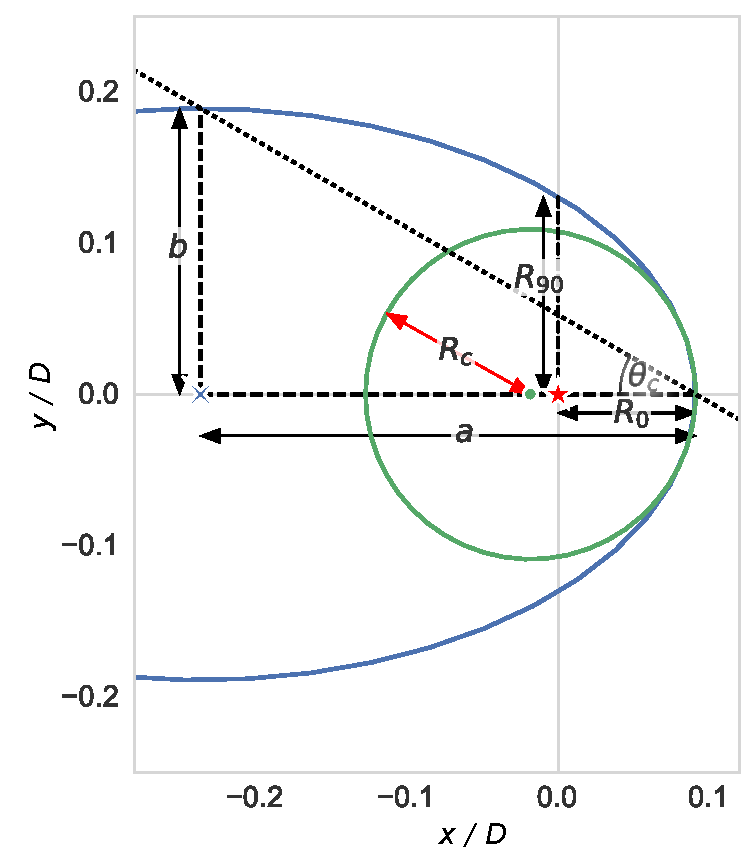
\includegraphics[width=0.4\linewidth]{./Figures/ellipse_edited} &
    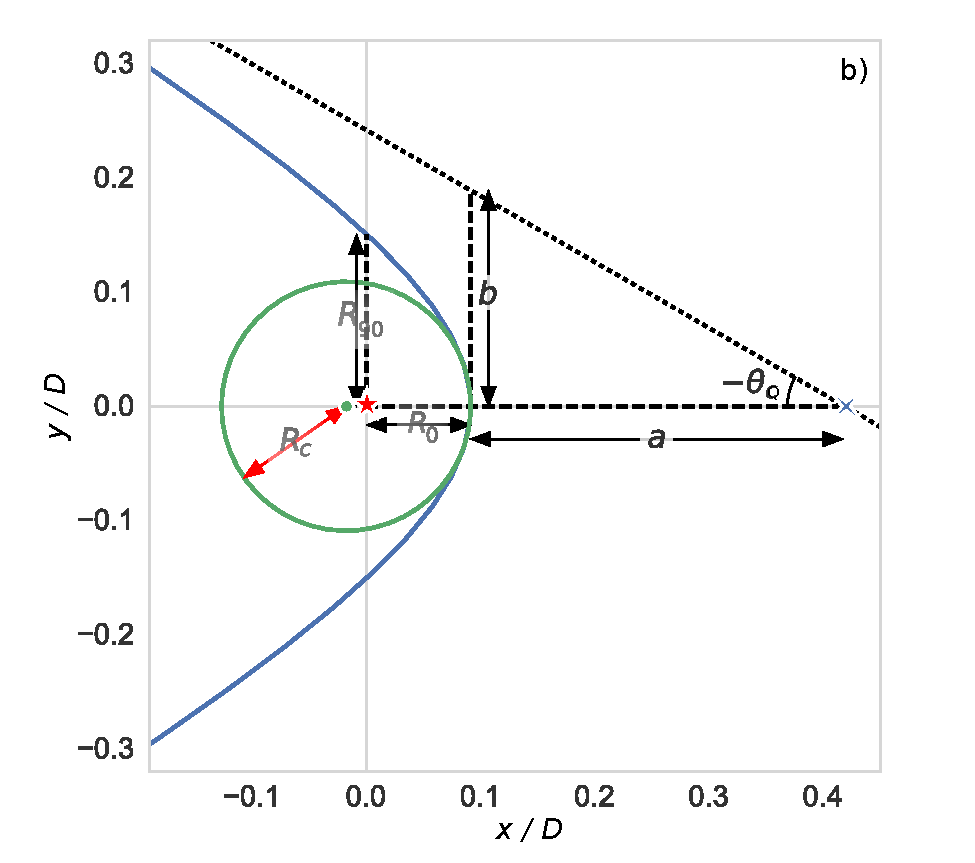
\includegraphics[width=0.5\linewidth]{./Figures/hyperbola_edited}
  \end{tabular}
  \caption{Representación esquemática de: Izquierda: Elipse. Y, derecha: Hipérbola. En ambos casos se ilustran los parámetros relevantes de éstas y los radios característicos}
  \label{fig:conics}
\end{figure}

\begin{figure}
  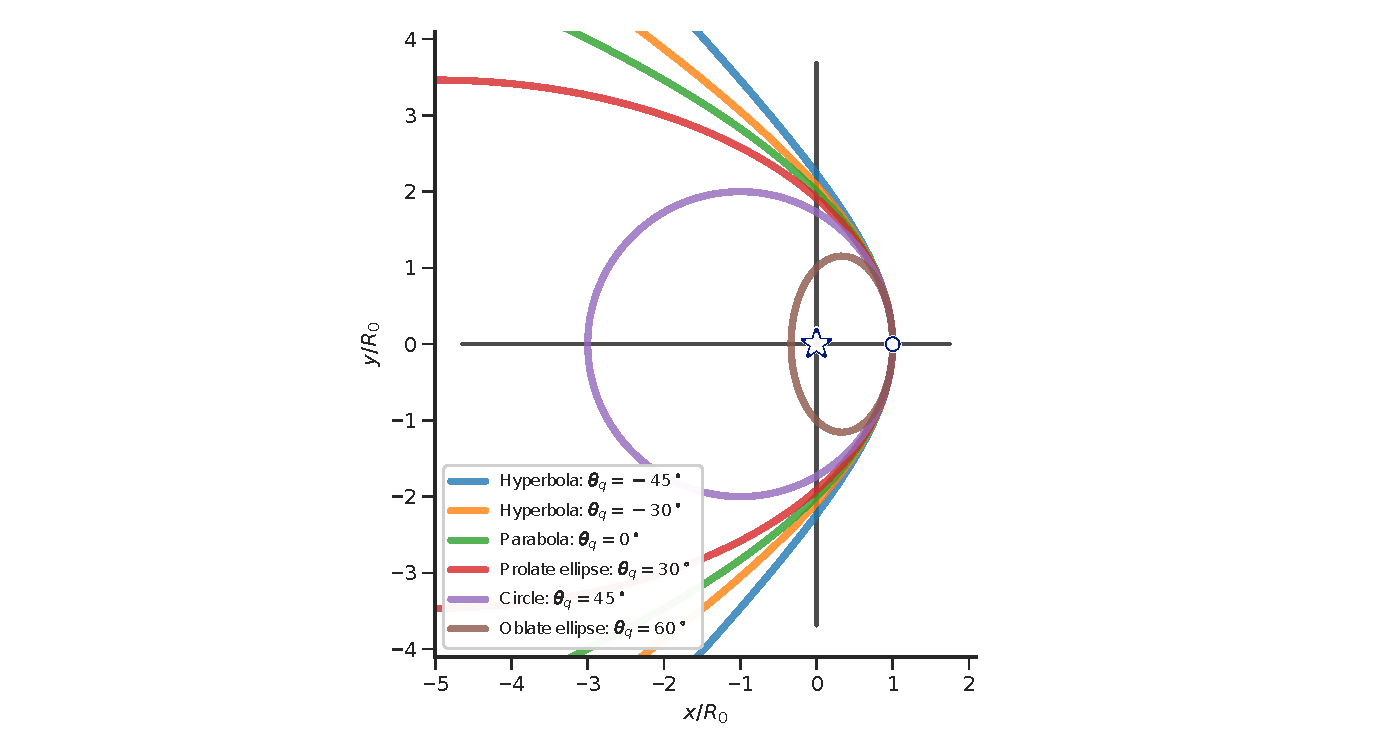
\includegraphics[width = 0.5\linewidth]{./Figures/conic1}
  \caption{Familia de curvas cónicas, donde el valor del parámetro $\theta_Q$ varía desde $\theta_Q < 0$ (hipérbolas) hasta $\theta_c > 0$ (elipses). Casos especiales son $\theta_Q = 0$ (parábola) y $\theta_Q = 45^\circ$ (círculo). Este parámetro sustituye en este trabajo a la excentricidad.}
  \label{fig:conics-family}
\end{figure}

%\subsection{Radios Característicos}
%\label{sec:conic-char-radii}
El set de parámetros $(a, x_0, \Q)$ es suficiente para caracterizar a nuestras cuádricas de revolución: $\Q$ nos indica el tipo de cónica, $a$ establece la escala y $x_0$ el desplazamiento del centro a lo largo del eje x. Sin embargo, para futuras aplicaciones tanto a modelos de interacción de vientos como a observaciones (capítulos \ref{chap:hipersonica} y \ref{chap:proplyds}) nos sería util hacer la caracterización mediante los parámetros $(R_0, \Pi, \Lambda)$ (ver \S \ref{sec:char-rad}). Las equivalencias entre los dos sets de parámetros los calculamos a continuación:

%Para que las curvas cónicas den una buena aproximación a la forma de un choque de proa dado, necesitamos saber calcular los radios característicos para éstas. A partir de la descripción de éstos en la \S \ref{sec:char-rad} podemos encontrar expresiones para cada uno de éstos en términos de los parámetros de las cónicas:

\begin{align}
  R_c &= \frac{b^2}{a} = a|\Q|\label{eq:R-curv-conic}\\
  R^2_{90} &= b^2\sigma\left(1 - \frac{x^2_0}{a^2}\right) = \Q\left(a^2 - x^2_0\right)\label{eq:R90-conic}
\end{align}

Combinando las ecuaciones (\ref{eq:x0})
%$R_0$ es independiente de los parámetros de las cónicas, por tanto, en esta sección nos será útil normalizar con este radio. De esta forma, podemos invertir las siguientes ecuaciones:

\begin{align}
  \tilde{a} &= \pm\frac{\tilde{R}_c}{2\tilde{R}_c - \tilde{R}_{90}^2} \label{eq:til-a}\\
  \tilde{b} &= \frac{\tilde{R}_c}{\left|2\tilde{R}_c - \tilde{R}_{90}^2\right|^{1/2}}\label{eq:til-b}\\
  \tan\theta_c &= \pm\left|2\tilde{R}_c - \tilde{R}_{90}^2\right|^{1/2} \label{eq:thc2}
\end{align}
Nótese que la cantidad $T_c\equiv 2\tilde{R}_c - \tilde{R}_{90}^2$ nos sirve como discriminante para distinguir el tipo de curva cónica que mejor ajusta a un choque de proa dado.

\subsection{Proyección en el plano del cielo}

El objetivo de esta sección es obtener la forma proyectada de las cuádricas de revolución, puesto que son una aproximación buena y mucho más sencilla a la forma real de un choque de proa. La forma tridimensional de las cuádricas de revolución viene dada por:

\begin{align}
  x &= a\Cos(t) + x_0 \\
  y &= b\Sin(t)\cos\phi \\
  z &= b\Sin(t)\sin\phi
\end{align}

Siguiendo el procedimiento mostrado en la \S \ref{sec:projection} calculamos el ángulo azimutal $\phi$ que cumple con el criterio de ser tangente al la línea de visión:

\begin{align}
  \sin\phi_T = \frac{b}{a}\tan i\Cot(t) 
\end{align}
Donde:
\begin{align}
  \Cot(t) = \left\lbrace
  \begin{array}{lr}
    \cot t & \mathrm{si}~\theta_c > 0 \\
    \coth t & \mathrm{si}~\theta_c < 0 
  \end{array}
  \right.
\end{align}

Ahora utilizamos la ecuación (\ref{eq:rotation}) para obtener la forma aparente de una cuádrica dada:

\begin{align}
  x'_T &= \frac{\Cos(t)}{a\cos i}\left(a^2\cos^2 i \pm b^2\sin^2 i\right) + x_0\cos i
  \label{eq:x-prime-proj}\\
  y'_T &= b\Sin(t)\left(1 - \frac{b^2}{a^2}\tan^2 i\Cot^2(t)\right)^{1/2}
  \label{eq:y-prime-proj}
\end{align}

Se espera que la forma proyectada de una cuádrica dada sea otra cuádrica del mismo tipo, por lo que es posible escribir las ecuaciones (\ref{eq:x-prime-proj}) y (\ref{eq:y-prime-proj}) de la siguiente manera: 

\begin{align}
  x'_T &= a'\Cos(t') + x'_0 \label{eq:xtprime}\\
  y'_T &= b'\Sin(t') \label{eq:ytprime}
\end{align}
Donde:
\begin{align}
  x'_0 &= x_0\cos i \\
  a' &= \left(a^2\cos^2 i \pm \b^2\sin^2 i\right)^{1/2} \label{eq:a-prime}\\
  b' &= b \label{eq:b-prime}\\
  \Cos(t') &= \frac{a'\Cos(t)}{a\cos i} \\
  \Sin(t') &= \left(1 - \Cos^2(t')\right)^{1/2}
\end{align}

Dos cantidades que nos van a ser de utilidad son los valores del parámetro $t$
que denominaremos $t_0$ y $t_{90}$ y son tales que $t'(t_0) = 0$ y $t'(t_{90}) = \frac{\pi}{2}$
o bien $y'_T(t_0) = 0$ y $x'_T(t_{90}) = 0$. De esta manera obtenemos las siguientes ecuaciones
implícitas evaluando las ecuaciones (\ref{eq:x-prime-proj}) y(\ref{eq:y-prime-proj}) en $t=t_{90}$
y $t=t_0$ respectivamente:

\begin{align}
  \Cot(t_0) &= \frac{a}{b}\cot{i} = \frac{\cot{i}}{\left|\tan\theta_c\right|} \label{eq:t0}\\
  \Cos(t_{90}) &= -\frac{ax_0\cos^2{i}}{a^2\cos^2{i}\pm b^2\sin^2{i}} \label{eq:t90}
\end{align}

Los radios característicos aparentes los podemos calcular a partir de las ecuaciones (\ref{eq:xtprime}) y
(\ref{eq:ytprime}) como se hizo para los radios característicos en el sistema no primado:

\begin{align}
  R'_0 &= \pm a' + x'_0\\
  R'_c &= \frac{b'^2}{a'}\\
  \tan\theta'_c &= \pm\frac{b'}{a'} \\
  R'_{90} &= \left(2R'_c \mp \tan^2\theta'_c\right)^{1/2}
\end{align}

Utilizando las ecuaciones (\ref{eq:x0}), (\ref{eq:a-prime}) y (\ref{eq:b-prime}),
utlizando la definición $D' = D\cos i$ e introduciendo la función
$f(i;\theta_c)\equiv \left(1 \pm \tan^2\theta_c\tan^2i\right)^{1/2}$ obtenemos
ecuaciones explícitas para los radios característicos en el sistema de referencia
del plano del cielo en términos de la inclinación:

\begin{align}
  \frac{q'}{q} &= 1 \pm \tilde{R}_c\cot^2\theta_c\left(f(i;\theta_c) - 1\right) \\
  \tilde{R}'_c &= \frac{\tilde{R_c}}{\cos^2if(i;\theta_c)\frac{q'}{q}} \label{eq:Rpc-quad}\\
  \tan\theta'_c &= \frac{\tan\theta_c}{\cos if(i;\theta_c)} \label{eq:thcp-quad}\\
  \tilde{R}'_{90} &= \left(\frac{2\tilde{R}_cf(i;\theta_c) \mp
                    \tan^2\theta_c\frac{q'}{q}}{q'/q}\right)^{1/2}\frac{\sec i}{f(i;\theta_c)}
                    \label{eq:Rp90-quad}
\end{align}

Cuando $\tilde{R}'_{90}$ es medible, entonces es posible hacer diagramas de diagnóstico como
el de la figura \ref{fig:diagnostic} para comparar con observaciones, independientemente de cualquier modelo de choques de proa.

\begin{figure}
  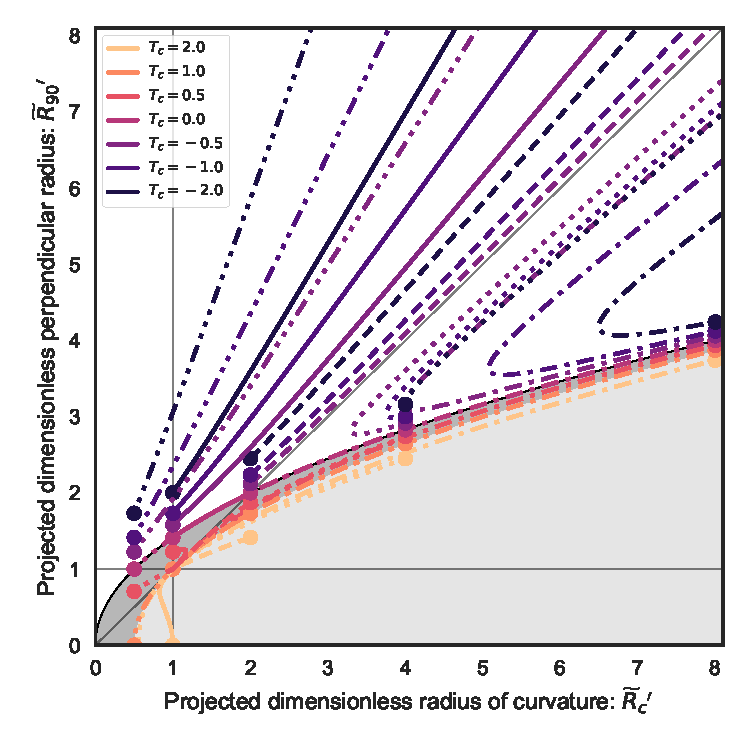
\includegraphics[width=0.5\linewidth]{./Figures/projected-R90-vs-Rc}
  \caption{Diagrama de diagnóstico $\tilde{R}'_{90}$ vs $\tilde{R}'_c$ para las cuádricas de revolución. En la región sin sombrear se representan las superficies abiertas (hiperboloides, $\theta_c <0$), mientras que la región más oscura representa a elipsoides prolatos  $(0 < \theta_c < 45^\circ)$ y la región poco sombreada a elipsoides oblatos $(\theta_c > 45^\circ)$}
  \label{fig:diagnostic}
\end{figure}

%Buscamos adjuntar el paper ``quadrics bowshock''
